\documentclass{article}
\usepackage[utf8]{inputenc}

\title{Lab9 - Creeping Line}
\author{Tsotne Putkaradze }
\date{May 2015}

\usepackage{natbib}
\usepackage{float}
\usepackage{graphicx}
\graphicspath{ {Pictures/} }
\usepackage{hyperref}
\begin{document}

\maketitle
\tableofcontents
\vspace{20mm} %just space

\listoffigures

\vfill
\section*{Introduction}
This document is created on a purpose of proving the understanding of blablabla

\clearpage
\section{Problem Statement}
The task given is following: we are required to write a single code, that will be uploaded to N number of FPGAs, which are connected with each other via serial connection, and which should construct marquee of text using existing Seven Segment Displays, in other words: moving text on Seven Segment Displays.
main things that should be considered \citep{digitalSystemsLab9}     

\begin{itemize}
     \item each FPGA should be able to be configured into Ma, Slave or By    pass mode: on run
     \item system should be scalable from 1     to N number of FPGAs
     \item we should provide some algorithm of error     checking (CRC, parity,..)
     \item there should be only one master in the whole chain, if there i    s more than one, stop process
     \item initialize some form of hand-shaking between FPGAs
\end{itemize}


\clearpage
\section{Solution}
Divide and Conquer ! 
In order to make life easy and things possible, we should break the whole system into smaller parts, design them : assemble.
We decided to use:
    \begin{itemize}
    \item Serial Connection
    \item one way Handshaking with header     
    \item CRC error checking
    \end{itemize}
For this methodology we created top module \href{/vhd/Creeping_Line_Serial.vhd}{Creeping Line Serial} which have following components:

\begin{enumerate}
  \item \href{run:./vhd/ReadingMemory.vhd}{Reading Memory}
    \begin{itemize}
        \item \href{run:./vhd/DataMemory.vhd}{Data Memory} 
        \item \href{run:./vhd/OutBuffer.vhd}{Output Buffer}
    \end{itemize}
  \item \href{run:./vhd/InBuffer.vhd}{Input Buffer}
  \item \href{run:./vhd/OutBuffer.vhd}{Output Buffer}
  \item \href{run:./vhd/SevSeg.vhd}{Seven Segment Controller}
  \item \href{run:./vhd/ClockStuff.vhd}{clock stuff}
  \item \href{run:./vhd/constr.ucf}{constraints} 
\end{enumerate}




\vfill
\subsection{General Description}
before we start describing each sub-part of system, lets talk about the behaviour of system, in general. data flow of system is following:
\begin{enumerate}
    \item we are waiting for header
    \item after getting right header we take input that is consisted of CRC code and actual data that should be printed
    \item we check CRC, if there is an error we changed damaged data with    bit-vector, that prints "dot" on seven segment display
    \item 
        \begin{itemize}
        \item we print data
        \item we shift data on seven segments
        \item we send old data on output
        \end{itemize}
\end{enumerate}

the general overview of system looks like this: 
\begin{figure}[H]
    \centering
   
 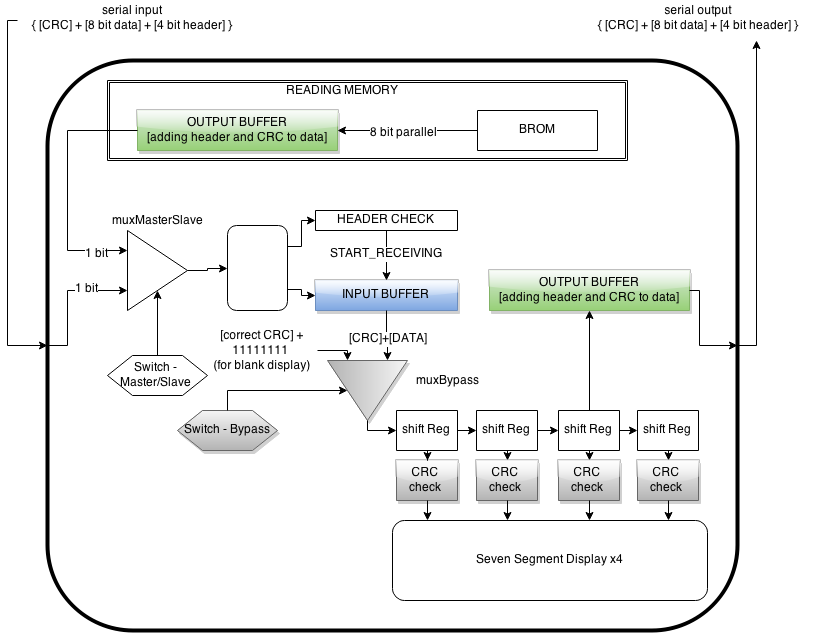
\includegraphics[scale=0.4]{CreepingLineDataFlow.png}
    \caption{Data Flow Diagram of Creeping Line}
    \label{fig:CreepingLineDataFlow}
\end{figure}


\vfill


\subsection{Input Buffer}

in input buffer element we have following inputs and output:
\begin{figure}[H]
    \centering
    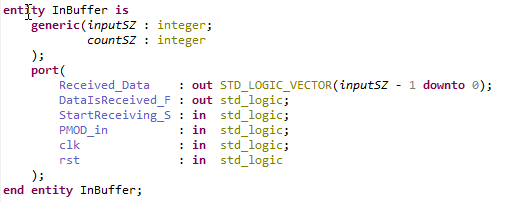
\includegraphics[scale=0.7]{InBuffer.png}
    \caption{Input Buffer ports}
    \label{fig:InBuffer}
\end{figure}
it takes input from PMOD and start signal, and and gives out received data with a flag notifying that data-reading-process has completed. please note that once start signal is given to the input buffer, nothing, except reset signal will affect/stop the process.

\subsection{Output Buffer}

in this buffer we have following ports
\begin{figure}[H]
    \centering
    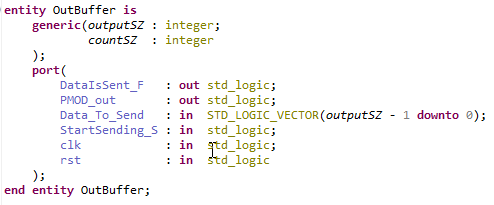
\includegraphics[scale=0.7]{OutBuffer.png}
    \caption{Output Buffer ports}
    \label{fig:OutBuffer}
\end{figure}

in this buffer, we take start signal and data that has a bitwidth of outputSZ, once we start outputting, the process can't be stopped.
but if we change "Data To Send" signal during the process, changed data will be send, this is because, otherwise we should have introduced another register with a size of outputSZ, that would get the value of "Data To Send" when Start signal would be 1, but i did not do that because it takes 1 clock cycle for this operation to start. but i wanted to make it in a way that, sending will start, immediately i provide the signal. the reason for that is Input buffer. lets say, we are reading header that was the one we expected, so then, next bit is data already, and that means, we should NOT introduce 1 clock cycle delay between header check and data reading, now, if we introduce this delay in output buffer, we can assume that, if:

\begin{itemize}
    \item receiving - takes 10 clock cycle
    \item sending - takes 10+1 clock cycle
\end{itemize}

so this creates imbalance and that might cause buffer overflow after some period of time. for example, if we have 100 clock cycles between sending of two data, in 100 clock cycle we will have buffer overflow.


\subsection{Reading Memory}
port description can be seen on the diagram below:
\begin{figure}[H]
    \centering
    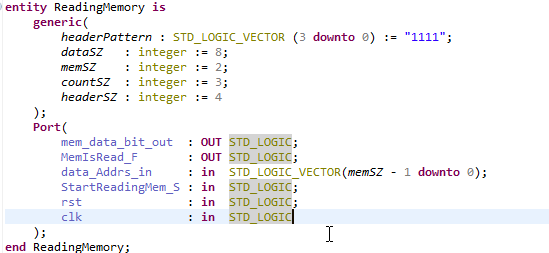
\includegraphics[scale=0.7]{ReadingMemory.png}
    \caption{Reading Memory ports description}
    \label{fig:ReadingMemory}
\end{figure}
in this module we have instantiated two components:
\begin{itemize}
\item Data Memory, that contains actual 8 bit data:
\begin{figure}[H]
    \centering
    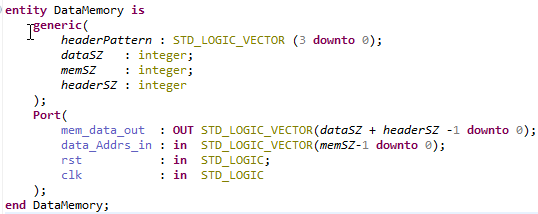
\includegraphics[scale=0.7]{DataMemory.png}
    \caption{Data Memory}
    \label{fig:DataMemory}
\end{figure}
\item and Output Buffer, that takes data from data memory and sends it bit-by-bit
\ref{fig:OutBuffer}
\end{itemize}
in this part, i tried to be smart and did following:
\begin{itemize}
\item created memory - i will make BROM later
\item and started to read data from memory in a linear way 
\end{itemize}
i did this because in this way, my data path will be same in both cases:
\begin{itemize}
\item if we are master and we are reading from memory
\item or if our board is in Slave mode, and we are just receiving data from PMOD
\end{itemize}
you can view the diagram here: \ref{fig:CreepingLineDataFlow}


\subsection{Other Elements}
in file 
\begin{itemize}
  \item \href{/vhd/SevSeg.vhd}{Seven Segment Controller} - we take four 8-bit inputs and print them on four seven segment displays
  \item \href{/vhd/ClockStuff.vhd}{clock stuff} - we take reference clock and generate every kind of clock we might ever need in our design:
  \begin{itemize}
  \item clock for Seven Segment Display
  \item clock for data transmission
  \item clock for button debouncer - in case we will use any buttons and etc.
  \end{itemize}
  \item \href{/vhd/constr.ucf}{constraints} - in this file we simply map our input-output ports on the pins of Nexys 3 board that has Spartan 6 FPGA.
    \item and finally, our top module looks like this:
    \begin{figure}[H]
    \centering
    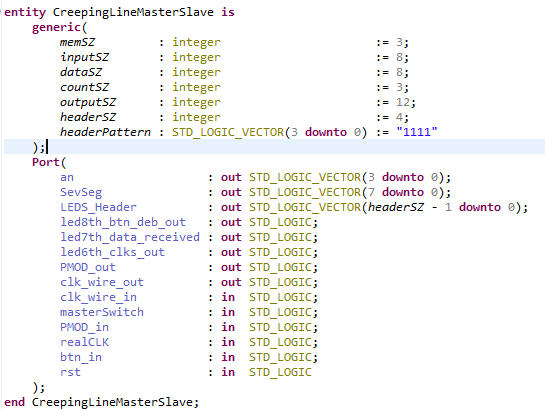
\includegraphics[scale=0.7]{CreepingLineMasterSlave.png}
    \caption{Creeping Line ports}
    \label{fig:CreepingLineMasterSlave}
\end{figure}
\end{itemize}

\section{Conclusion / Results}
Benefits, Results and Conclusions from this project are following:
\begin{enumerate}
\item understanding the principles of Serial Communication
\item principles, drawbacks and benefits of handshake communication
\item importance of synchronous operations, data-sending and receiving cycles/times
\end{enumerate}

\bibliographystyle{plain}
\bibliography{references}






\end{document}
